\documentclass[../basicOrbitalDynamics.tex]{subfiles}
\graphicspath{{\subfix{../images/}}}
\begin{document}

\bigskip\bigskip

\subsection{Orbit Planar Geometry}

\begin{figure}[H]
    \centering
    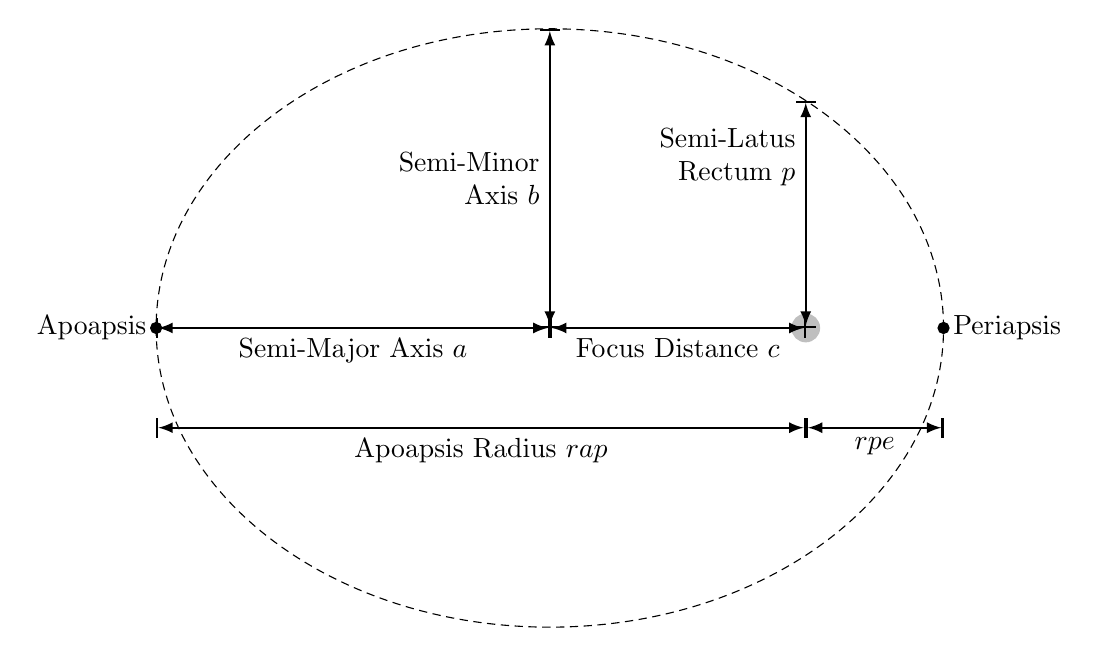
\begin{tikzpicture}[>=latex]
        \def\ecc{0.65}
        \def\SMA{5}
        \def\ap{\fpeval{\SMA*(1+\ecc)}}
        \def\pe{\fpeval{\SMA*(1-\ecc)}}
        \def\slr{\fpeval{\SMA*(1-(\ecc)^2)}}
        \def\SmA{\fpeval{\SMA*(1-(\ecc)^2)^(1/2)}}

        \draw[thin, densely dashed] (0,0) ellipse ({\SMA} and {\SmA});
        \filldraw[lightgray] (\ap-\SMA,0) circle (5pt);

        \draw[|<->|, thick] (-\SMA, 0) -- (0, 0) node[midway, below] {Semi-Major Axis $a$};
        \draw[|<->|, thick] (0, 0) -- (0, \SmA) node[align=right, midway, left] {Semi-Minor\\Axis $b$};
        \draw[|<->|, thick] (\ap-\SMA, 0) -- (\ap-\SMA, \slr) node[align=right, near end, left] {Semi-Latus\\Rectum $p$};

        \draw[|<->|, thick] (0,0) -- (\ap-\SMA,0) node[midway, below] {Focus Distance $c$};

        \draw[|<->|, thick] (\ap-\SMA, -\SmA/3) -- (\SMA, -\SmA/3) node[midway, below] {$\st{r}{pe}$};

        \draw[|<->|, thick] (-\SMA, -\SmA/3) -- (\ap-\SMA, -\SmA/3) node[midway, below] {Apoapsis Radius $\st{r}{ap}$};

        \filldraw[] (\SMA,0) circle (2pt) node[right] {Periapsis};
        \filldraw[] (-\SMA,0) circle (2pt) node[left] {Apoapsis};

    \end{tikzpicture}

    \caption{An orbit with important geometric values labeled}\label{fig:Orbit Diagram}
\end{figure}

In the above figure, the semi-major axis $a$, semi-minor axis $b$, semi-latus rectum $p$, focus distance $c$, apoapsis radius $\st{r}{ap}$, and periapsis radius $\st{r}{pe}$ are all labeled. The apoapsis is the highest point in the orbit, and the periapsis is the lowest. The major axis is the largest distance across the ellipse, while the minor axis is the smallest. The latus rectum is the width of the ellipse perpendicular to the foci. The focus distance is the distance between the foci and the center of the ellipse.


\bigskip\bigskip
\subsection{Positional Diagram}
\begin{figure}[H]
    \centering
    \includegraphics[scale=0.1]{WikiImage}
    \caption{Figure from wikipedia.org showing orbital elements}\label{fig:Wiki Image}
\end{figure}
There are a variety of parameters that are used to position the orbit in space, and to position the satellite in the orbit. Note that $\nu$ (nu) and $\theta$ (theta) are used interchangeably, with $\theta$ being used predominantly in this document. The blue line points to the periapsis. Note also that the blue line and the red line are not necessarily aligned with eachother.

The base frame $a$ can be defined such that $\hat{a}_1$ points in the reference direction, $\hat{a}_2$ points 90 degrees clockwise of the reference direction in place with the reference plane, and $\hat{a}_3$ pointing normal to the base frame (generally ``up'' in the image above).

Another frame $b$ can be defined such that $b$ is the same as the $a$ frame, but rotated $\Omega$ about $\hat{a}_3$. This means that $\hat{b}_1$ points toward the ascending node, $\hat{b}_2$ is normal to $\hat{b}_1$ and in the reference plane, and $\hat{b}_3=\hat{a}_3$.

Frame $c$ can be defined as a rotation of frame $b$ about $\hat{b}_1$ by $i$. This frame is in the plane of the orbit, with $\hat{c}_1=\hat{b}_1$ and $\hat{c}_3$ being normal to the orbit.

Next, $d$ can be defined as a rotation of $c$ by $\omega$ about $\hat{c}_3$. This frame is also in the plane of the orbit, with $\hat{c}_1$ pointing toward the periapsis.

Finally, another frame can be defined as a rotation of $d$ by $\theta$ about $\hat{d}_3$. This creates the polar frame (see Figures \ref{fig:Coordinate System} and \ref{fig:Coordinate System 3D}).

\begin{figure}[H]
    \centering
    \includegraphics[scale=0.3]{Frames}
    \caption{Reference frames (aside from polar and maneuvering frames)}\label{fig:Frames}
\end{figure}

To get a better sense for how orbital parameters work, it is highly reccomended that the reader experiment with https://orbitalmechanics.info/

\bigskip\bigskip
\subsection{Orbit elements}

\begin{comment}
\begin{figure}[H]
    \centering
    \def\SMA{3}
    \def\inc{20}

    \tdplotsetmaincoords{70}{40}
    \begin{tikzpicture}[tdplot_main_coords, >=latex]
        \tdplotsetrotatedcoords{0}{-\inc}{0}

        %original orbit
        \draw[lightgray, samples=250, red] plot ({deg(\x)}:\SMA);
        \draw[red, ->] (0,0,0) -- +(\SMA,0,0);
        \draw[red, ->] (0,0,0) -- +(0,0,1);

        % inclined orbit
        \draw[tdplot_rotated_coords, samples=250] plot ({deg(\x)}:\SMA);
        \draw[tdplot_rotated_coords, ->] (0,0,0) -- +(\SMA,0,0);
        \draw[tdplot_rotated_coords, ->] (0,0,0) -- +(0,0,1);

        % Ascending an Descending Nodes
        \filldraw[] (0,\SMA,0) circle (1pt) node[above right, black] {\small DN};
        \filldraw[] (0,-\SMA,0) circle (1pt) node[below left, black] {\small AN};
        \draw[densely dashed] (0,\SMA,0)--(0,-\SMA,0);
        \draw[densely dashed] (2,0,0) arc (0:270:2) node[near end, above] {$\Omega$};

        % inclination labels
        \draw[tdplot_rotated_coords,gray, densely dashed] (0,0,0) -- +(0,0,2);
        \draw[densely dashed, gray] (0,0,0) -- (0,0,2);
        \tdplotsetrotatedcoords{-90}{90}{90}
        \draw[tdplot_rotated_coords, densely dashed, thick] (0,2,0) arc (90:90+\inc:2) node[midway, above] {$i$};
        \draw[tdplot_rotated_coords, densely dashed, thick] (\SMA,0, 0) arc (0:\inc:\SMA) node[midway, right] {$i$};
    \end{tikzpicture}
    \caption{An orbit with inclination and longitude of ascending node shown}\label{fig:Inclination}
\end{figure}

The inclination $i$ is shown in the above figure, as well as both the ascending and descending nodes. The longitude of ascending node $\Omega$ is shown as well, which in this case is 270 degrees.
\end{comment}

\begin{figure}[H]
    \centering
    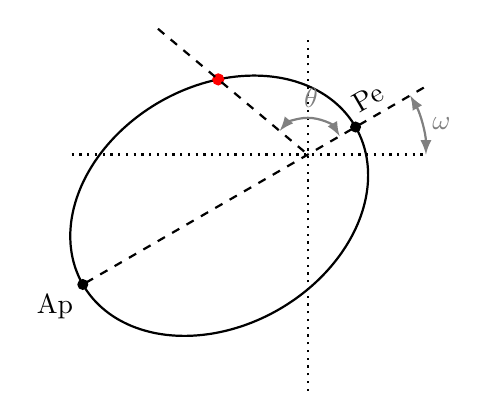
\begin{tikzpicture}[>=latex]
        \def\ecc{0.65}
        \def\SMA{2}
        \def\ap{\fpeval{\SMA*(1+\ecc)}}
        \def\pe{\fpeval{\SMA*(1-\ecc)}}
        \def\omeg{30}
        \def\slr{\fpeval{\SMA*(1-\ecc^2)}}
        \def\arcRad{1.5}
        \def\thta{110}

        \draw[thick, dotted] (-3,0)--(1.5,0);
        \draw[thick, dotted] (0,-3)--(0,1.5);
        \draw[domain=0:2*pi,samples=500, thick] plot ({deg(\x)+\omeg}:{(\slr)/(1+\ecc*cos(\x r))});
        \draw[thick, dashed] (\omeg:\pe+\SMA/2)--(180+\omeg:\ap);
        \draw[thick, <->, gray] (\arcRad,0) arc (0:\omeg:\arcRad) node[midway, right] {$\omega{}$};

        \fill(\omeg: -\ap) circle (2pt) node[below left] {Ap};

        \fill(\omeg: \pe) circle (2pt) node[anchor=center, rotate=\omeg, above right] {Pe};
        \filldraw[red] (\omeg+\thta: \fpeval{\slr/(1+\ecc*cos(deg(\thta)))}) circle (2pt);

        \draw[thick, dashed] (\omeg+\thta:\fpeval{\slr/(1+\ecc*cos(deg(\thta)))}+\SMA/2)--(0,0);
        \draw[thick, <->, gray] (\omeg:2*\pe/3) arc (\omeg:\thta+\omeg:2*\pe/3) node[midway, above] {$\theta$};

    \end{tikzpicture}

    \caption{True Anomaly and Argument of Periapsis}\label{fig:True Anomaly and Arg of Periapsis}
\end{figure}
Above, an orbit is shown with the major axis indicated by a dashed line, and the apoapsis (Ap) and periapsis (Pe) labeled. The origin of this coordinate system is the focus about which the body orbits. The argument of periapsis $\omega$ is the angle between the periapsis of the orbit and the ascending node (the +x axis in this case), and the true anomaly $\theta$ (sometimes designated $\nu$) is the angle between the satellite's current location and its periapsis

\bigskip\bigskip
\subsection{Coordinate Systems}
\begin{figure}[H]
    \centering
    \begin{tikzpicture}[>=latex]
        \def\dist{1.5}
        \def\thta{75}
        \def\unMag{1}
        \def\arcRad{1.5}
        \def\phiAng{25}
        \def\vMag{2}

        \coordinate (rOffs) at (5, 0) {};
        \coordinate (pt) at (\thta:\dist) {};

        \filldraw[] (pt) circle (2pt);

        \draw[dotted] (0,0) -- (pt);
        \draw[densely dashed, -{Latex[open]}, lightgray, ultra thick] (pt) -- +(\thta:\unMag) node[right] {$\hat{u}_r$};
        \draw[densely dashed, -{Latex[open]}, lightgray, ultra thick] (pt) -- +(\thta+90:\unMag) node[below] {$\hat{u}_\theta$};

        \draw[->] (pt) --+(\thta-\phiAng-90:\vMag/2) --+(\thta-\phiAng+90:\vMag)node[left] {$\vv{v}$};

        \draw[->, gray] (pt)+(\thta+90:\arcRad) arc (\thta+90:\thta+90-\phiAng:\arcRad) node[midway, left] {$\phi$};

        \node[circle, fill=white, draw=black] at (0,0) {};
    \end{tikzpicture}
    \qquad
    \begin{tikzpicture}[>=latex]
        \def\dist{1.5}
        \def\thta{75}
        \def\unMag{1}
        \def\arcRad{1.5}
        \def\phiAng{25}
        \def\vMag{2}

        \coordinate (rOffs) at (5, 0) {};
        \coordinate (pt) at (\thta:\dist) {};

        \filldraw[] (pt) circle (2pt);

        \draw[dotted] (0,0) -- (pt);
        \draw[densely dashed, -{Latex[open]}, lightgray, ultra thick] (pt) -- +(\thta-\phiAng:\unMag) node[right] {$\hat{m}_r$};
        \draw[densely dashed, -{Latex[open]}, lightgray, ultra thick] (pt) -- +(\thta-\phiAng+90:\unMag) node[below] {$\hat{m}_v$};

        \draw[->] (pt) --+(\thta-\phiAng-90:\vMag/2) --+(\thta-\phiAng+90:\vMag)node[left] {$\vv{v}$};

        \draw[->, gray] (pt)+(\thta+90:\arcRad) arc (\thta+90:\thta+90-\phiAng:\arcRad) node[midway, left] {$\phi$};

        \node[circle, fill=white, draw=black] at (0,0) {};
    \end{tikzpicture}

    \caption{Polar and maneuvering vector frames}\label{fig:Coordinate System}
\end{figure}

A satellite (black dot) is shown orbiting a source (hollow circle) with the flight path angle $\phi$ and velocity vector $\vec{v}$ indicated. On the left image, the polar basis vectors $u$ are shown. On the right, the manuevering vectors $m$ are shown.

The polar basis vectors are defined such that $\hat{u}_r$ points radially outward from the planet, with $\hat{u}_\theta$ being perpendicular to it and generally in the direction of the velocity vector (and in plane with both $\vec{v}$ and $\hat{u}_r$). $\hat{u}_n$ is defined $\hat{u}_n=\hat{u}_r\times\hat{u}_\theta$. In this figure, $\hat{u}_n$ points out-of-page.

The manuevering basis vectors $m$ are defined such that $\hat{m}_v$ points in the direction of the velocity, with $\hat{m}_r$ being normal to it and generally facing away from the planet (and in the plane defined by the velocity vector and the planet). $\hat{m}_n$ will always be equal to $\hat{u}_n$, and is defined as $\hat{m}_n=\hat{m}_r\times\hat{m}_v$.

The flight path angle is the angle between the two basis vectors

\bigskip\bigskip
\subsection{Coordinate System 3D}
\begin{figure}[H]
    \centering
    \def\ecc{0.65}
    \def\SMA{3}
    \def\slr{\fpeval{\SMA*(1-\ecc^2)}}
    \def\ap{\fpeval{\SMA*(1+\ecc)}}
    \def\pe{\fpeval{\SMA*(1-\ecc)}}
    \def\dst{\ap}
    \def\SmA{\fpeval{\SMA*sqrt(1-\ecc^2)}}
    \def\inc{20}

    \tdplotsetmaincoords{70}{30}
    \begin{tikzpicture}[tdplot_main_coords, >=latex]
        \draw[->, green, ultra thick] (0,0,0) -- (2,0,0);
        %\draw[->, red] (0,0,0) -- (0,1,0) node[above]{$y$};
        %\draw[->, red] (0,0,0) -- (0,0,1) node[above]{$z$};
        \draw[densely dashed, gray] (0,0,0) -- (\fpeval{\dst*cos(deg(\inc))},0,0)--+(0,0,\fpeval{\dst*sin(deg(\inc))});

        \tdplotsetrotatedcoords{0}{-\inc}{0}
        \coordinate[tdplot_rotated_coords] (pt) at (3,0,0);

        % orbit
        \draw[tdplot_rotated_coords,samples=500, lightgray] plot ({deg(\x)}:{(\slr)/(1-\ecc*cos(\x r))});
        \draw[tdplot_rotated_coords, gray] (-\pe,0,0) -- (\ap,0,0);
        \draw[tdplot_rotated_coords, gray] (\ecc*\SMA,-\SmA,0) -- (\ecc*\SMA,\SmA,0);

        % Ascending an Descending Nodes
        \filldraw[red] (0,\slr,0) circle (1pt) node[right, black] {\small DN};
        \filldraw[red] (0,-\slr,0) circle (1pt) node[left, black] {\small AN};
        \draw[dotted, red] (0,\slr,0)--(0,-\slr,0);


        % new coord system
        \draw[tdplot_rotated_coords,blue, ->] (\dst,0,0) -- +(1,0,0) node[right]{$\hat{u}_r$};
        \draw[tdplot_rotated_coords,blue, ->] (\dst,0,0) -- +(0,1,0) node[above right]{$\hat{u}_\theta$};
        \draw[tdplot_rotated_coords,blue, ->] (\dst,0,0) -- +(0,0,1) node[above]{$\hat{u}_n$};
        \filldraw[tdplot_rotated_coords] (\dst,0,0) circle (2pt);

        % Inclination Label
        \draw[tdplot_rotated_coords,blue, ->] (0,0,0) -- +(0,0,1) node[left]{$\hat{u}_n$};
        \draw[tdplot_rotated_coords,gray, densely dashed] (0,0,0) -- +(0,0,2);
        \draw[densely dashed, gray] (0,0,0) -- (0,0,2);
        \tdplotsetrotatedcoords{-90}{90}{90}
        \draw[tdplot_rotated_coords, densely dashed, thick] (0,2,0) arc (90:90+\inc:2) node[midway, above] {$i$};
    \end{tikzpicture}

    \caption{Inclined orbit showing the polar basis vectors}\label{fig:Coordinate System 3D}
\end{figure}
A satellite (black dot) is shown above orbiting a body with the polar coordinate system shown. The semi-major and semi-minor axes are shown with a thin line. Note that in this position (at the apoapsis in this case, however this also holds true at periapsis), the polar $u$ and maneuvering $m$ basis vectors are equal.

Note that the inclination $i$ of the orbit is also shown. In this figure the satellite is shown with $\theta=\pi$ and $\omega=\frac{3}{2}\pi$ (the satellite is 180 degrees offset from its periapsis, and the periapsis is 270 degrees offset from the ascending node). The red dots are the ascending and descending nodes. These are the points at which the orbit intersects the horizon. The ascending node (AN) is the one at which the latitude changes from negative to positive, and the desending node (DN) is the point at which latitude goes from positive to negative. In this figure, $\Omega=\frac{3}{2}\pi$ (with the reference direction being the green arrow). Note that $\Omega$ does not always equal $\omega$; $\Omega$ positions the ascending node relative to a reference direction, while $\omega$ positions the periapsis relative to the ascending node.

\end{document}